\usepackage{tikz}
\usetikzlibrary{arrows.meta,positioning}
\tikzset{
  node/.style={draw, rounded corners, align=center, inner sep=3pt},
  latent/.style={draw, dashed, rounded corners, align=center, inner sep=3pt},
  fe/.style={draw, dotted, rounded corners, align=center, inner sep=3pt},
  ->/.style={-{Latex[length=2mm]}, line width=0.6pt}
}

\begin{figure}[!ht]
\centering
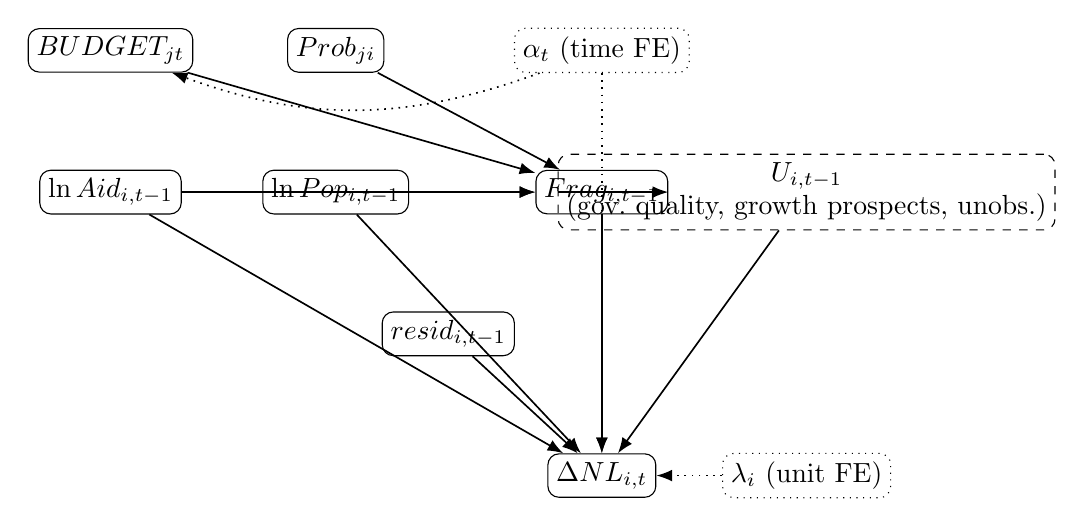
\begin{tikzpicture}[x=1.3cm,y=1.2cm]

% Row 1: instruments and shocks
\node[node] (B) at (0,3) {$BUDGET_{j t}$};
\node[node] (P) at (2.2,3) {$Prob_{j i}$};
\node[fe]   (Alpha) at (4.8,3) {$\alpha_t$ (time FE)};

% Row 2: controls and endogenous regressor (t-1)
\node[node] (Aid) at (0,1.5) {$\ln Aid_{i,t-1}$};
\node[node] (Pop) at (2.2,1.5) {$\ln Pop_{i,t-1}$};
\node[node] (Frag) at (4.8,1.5) {$Frag_{i,t-1}$};

% Row 3: residual CF and outcome
\node[node] (Resid) at (3.3,0) {$resid_{i,t-1}$};
\node[node] (Delta) at (4.8,-1.5) {$\Delta NL_{i,t}$};

% Latent + unit FE
\node[latent] (U) at (6.8,1.5) {$U_{i,t-1}$ \\ (gov.\ quality, growth prospects, unobs.)};
\node[fe]     (Lambda) at (6.8,-1.5) {$\lambda_i$ (unit FE)};

% Arrows: instruments -> Frag
\draw[->] (B) -- (Frag);
\draw[->] (P) -- (Frag);

% Exclusion (no direct path B/P -> DeltaNL): encoded by absence of edges

% Controls
\draw[->] (Aid) -- (Frag);
\draw[->] (Aid) -- (Delta);
\draw[->] (Pop) -- (Frag);
\draw[->] (Pop) -- (Delta);

% Endogenous -> Outcome
\draw[->] (Frag) -- (Delta);

% Control-function residual -> Outcome
\draw[->] (Resid) -- (Delta);

% Latent confounding paths
\draw[->] (U) -- (Frag);
\draw[->] (U) -- (Delta);

% Fixed effects as absorbers (dotted incoming to both sides)
\draw[->, dotted] (Alpha) -- (Delta);
\draw[->, dotted] (Lambda) -- (Delta);

% Optional dotted absorption of common shocks into Budget as a reminder
\draw[->, dotted] (Alpha) to[bend left=20] (B);

% Layout helpers: (not strictly necessary)
% \draw[help lines] (-0.5,-2.5) grid (8,3.5);

\end{tikzpicture}
\caption{Causal DAG for instrumented fragmentation and night-lights outcome. 
$BUDGET_{jt}\times Prob_{ji}$ enters estimation as an interaction (the IV), 
here represented by separate arrows into $Frag_{i,t-1}$. Exclusion requires no direct 
$BUDGET_{jt}$ or $Prob_{ji}$ effect on $\Delta NL_{i,t}$ except through $Frag_{i,t-1}$. 
Control-function adds $resid_{i,t-1}$ to the outcome to net out endogeneity. 
$\alpha_t$ and $\lambda_i$ denote absorbed time and unit fixed effects.}
\end{figure}
